\section{Conclusion and Future Work}
We present a compact representation of PRT for \textbf{free form} deformable objects, in form of a non-linear model, namely a deep convolutional neural network.  The model is able to extract the features of the dataset relevant to self-shadowing and thus generate good approximations for a wide spectrum of deformations. The results show that our CNN is able to faithfully predict appearances that are visually undistinguishable from the ground truth.  With this in mind we showed that compared to traditional PRT methods, DeepPRT leads to immense memory savings.
\\ 
Moreover, our method shows much higher generalisation properties than previous approaches allowing deformations from much larger and less constrained deformation spaces.\\
\\
Although we showed DeepPRT can be much more compact than traditional PRT, our network is far from being optimal. Network optimisation methods would enhance our DeepPRT approach significantly \cite{Survey_NN_Compression}, \cite{Deep_Compression}.
Moreover, other network topologies and/or cost functions could be explored in order to achieve  better approximations, for instance, the use of deformable convolutions \cite{DeformableCNN} to account for individual object deformations could be explored, as proposed in \cite{Deformable_UNet}.
\\
The particular choice of our basis functions (\textit{Spherical Harmonics}), currently restricts our method to low-frequency lightings. However, an extension to all-frequencies is possible by fitting the model to an alternative representation of $T$, such as non-linear Wavelets \cite{AllFrequencyPRT}.
\\
The most significant limitations of our method reside within the choice of our parametrisation (Harmonic Map) and the natural flaws of the geometry images surface representation.  Currently, DeepPRT only performs well for modest curvature variations and is restricted to surfaces with one boundary (topological disks); however, using the \textit{Strech-Minimising} parametrisation instead and further using the extension proposed by \cite{Spherical_Parametrization}, the shape representation would be more robust and our method would be applicable to more general surface shapes. \\
Apart from that, alternative surface representations could be explored to overcome this restrictions natural flaws of \textit{geometry images}. 
\begin{figure*}
  \centering
    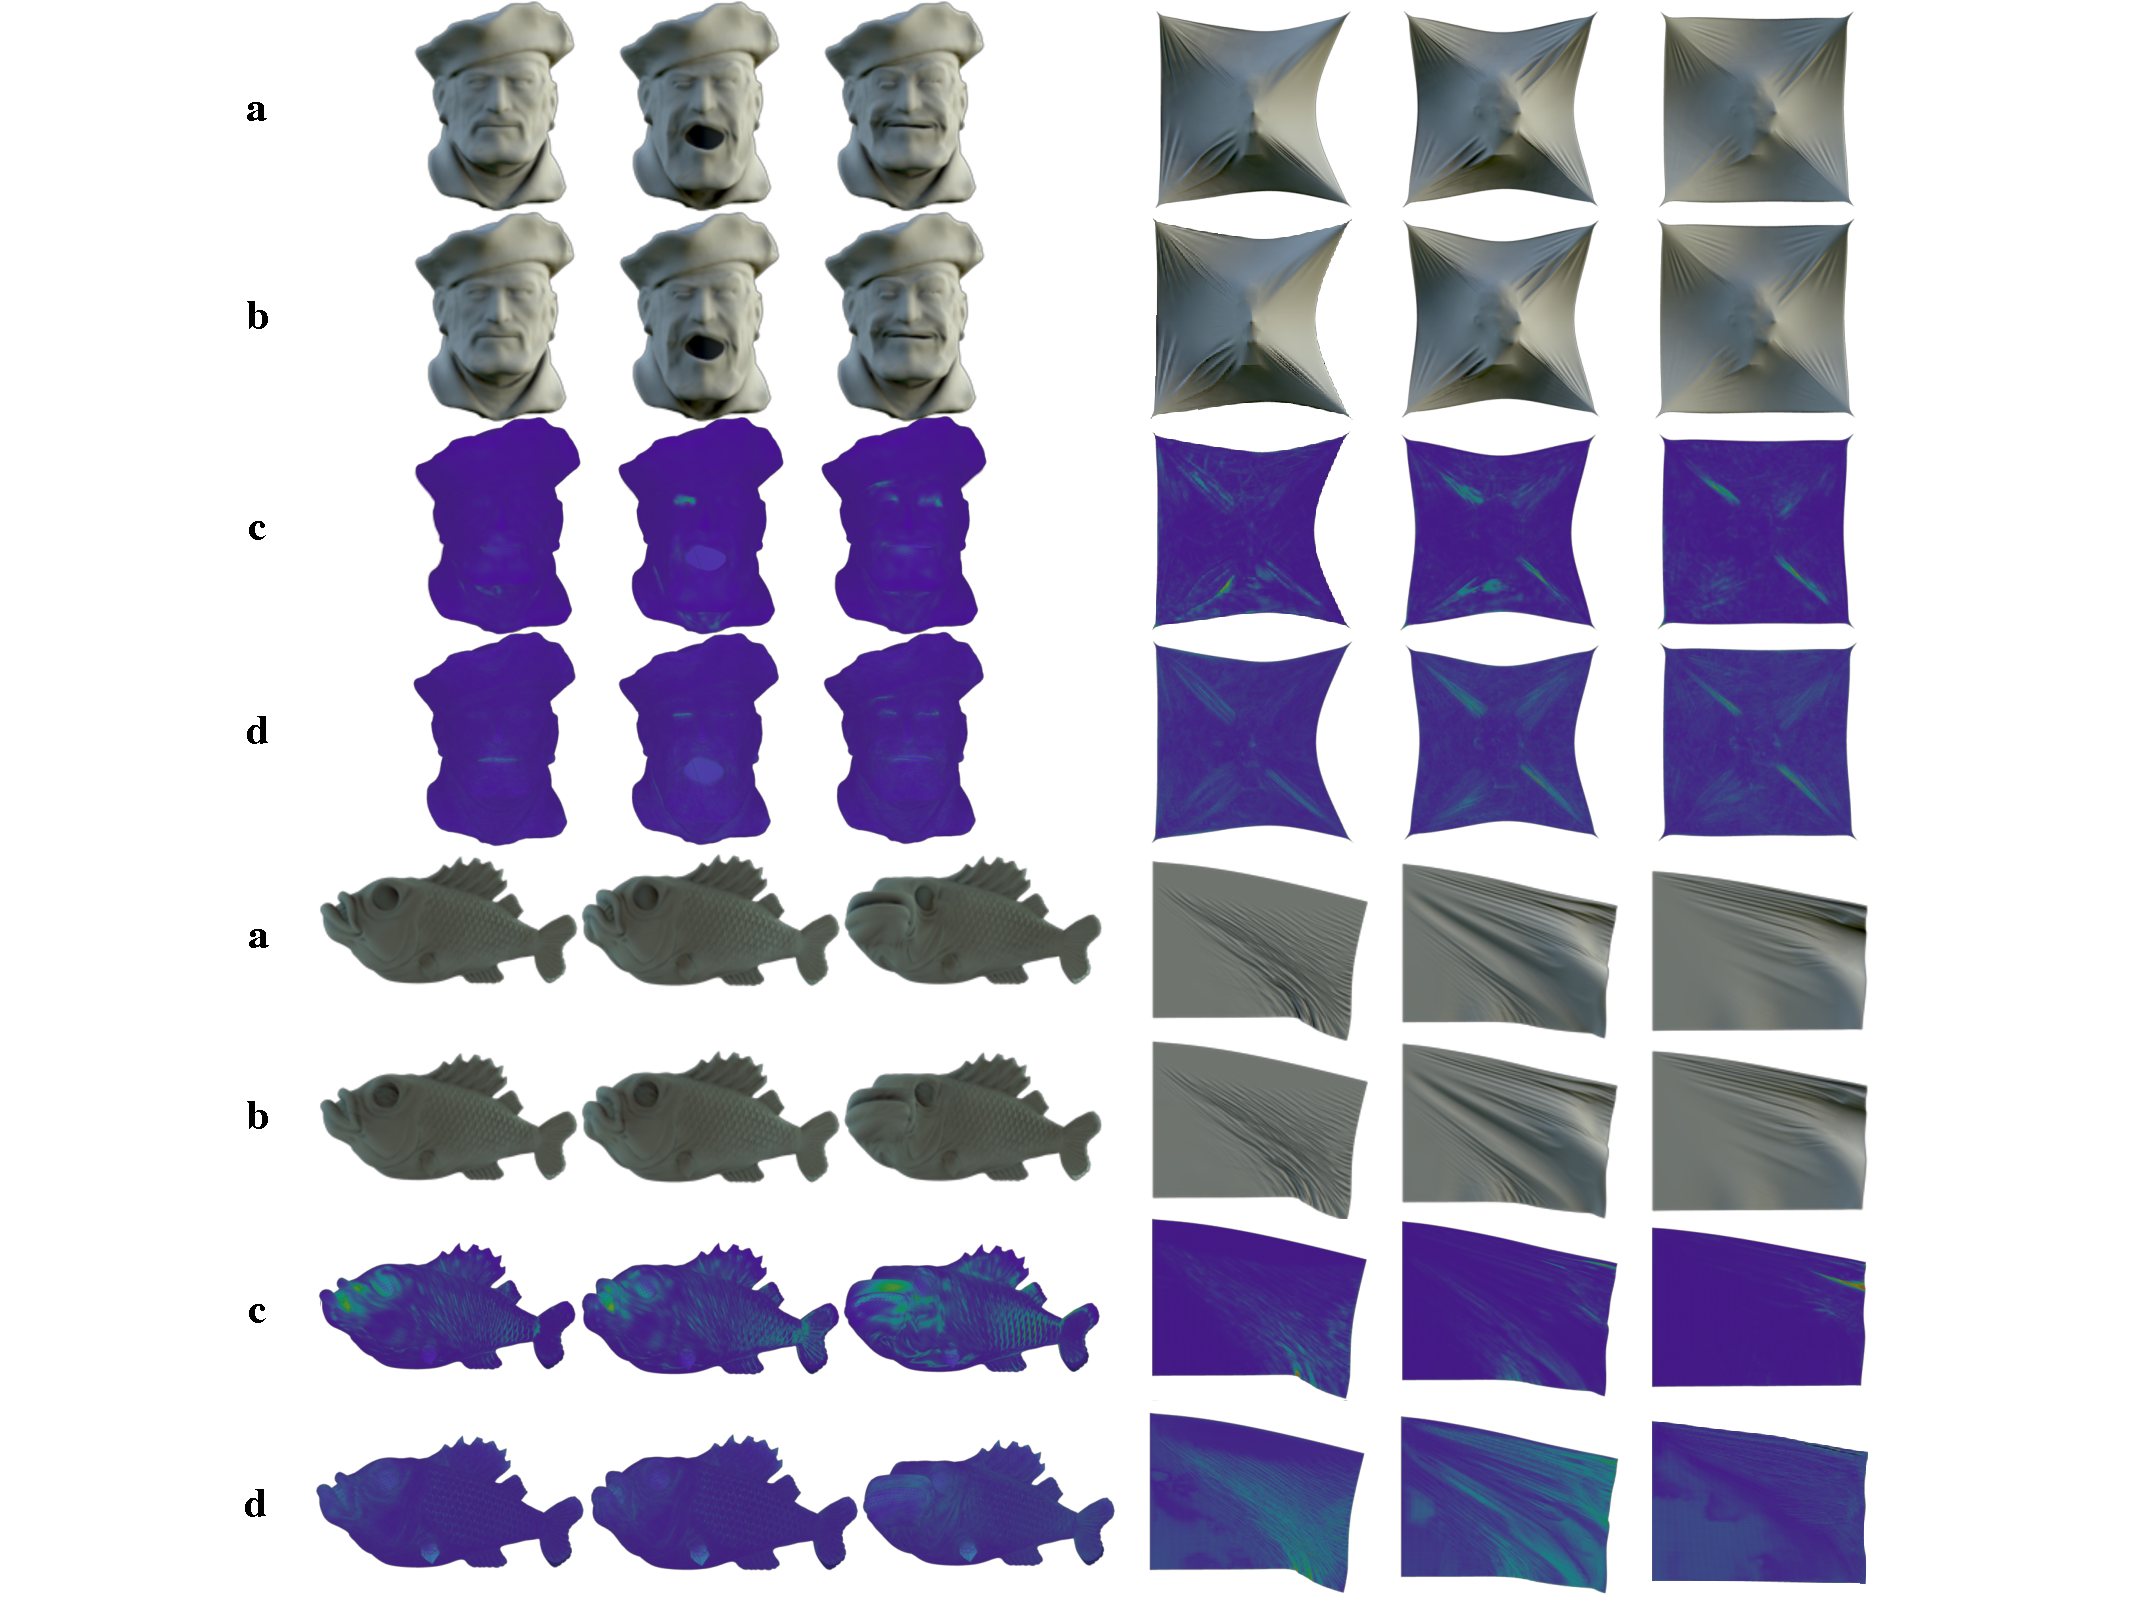
\includegraphics[width=0.7\paperwidth]{Figures/DPRT_quality_SSIM.pdf}
     \caption{Visual Quality:
     a : Ground truth appearance. b: CNN appearance prediction. c: SSIM. d: L1-Error between ground truth and predicted transfer coefficients }
     \label{Fig: DPRT_Quality}
\end{figure*}